\documentclass{warpdoc}
\newlength\lengthfigure                  % declare a figure width unit
\setlength\lengthfigure{0.158\textwidth} % make the figure width unit scale with the textwidth
\usepackage{psfrag}         % use it to substitute a string in a eps figure
\usepackage{subfigure}
\usepackage{rotating}
\usepackage{pstricks}
\usepackage[innercaption]{sidecap} % the cute space-saving side captions
\usepackage{scalefnt}

%%%%%%%%%%%%%=--NEW COMMANDS BEGINS--=%%%%%%%%%%%%%%%%%%%%%%%%%%%%%%%%%%
\newcommand{\alb}{\vspace{0.2cm}\\} % array line break
\newcommand{\Cp}{{C_{P}}}
\newcommand{\nd}{{n_{\rm d}}}
\newcommand{\nf}{{n_{\rm f}}}
\newcommand{\ns}{{n_{\rm s}}}
\newcommand{\CFL}{{\rm CFL}}
\newcommand{\bb}{{b_b}}
\newcommand{\br}{{b_r}}
\newcommand{\loope}{{\rm e}}
\newcommand{\loops}{{\rm s}}
\newcommand{\loopE}{{\rm E}}
\newcommand{\loopS}{{\rm S}}
\newcommand{\xiverge}{{\xi_{\rm verge}}}
\newcommand{\varphiverge}{{\varphi_{\rm verge}}}
\newcommand{\ximax}{{\xi_{\rm max}}}
\newcommand{\turb}{_{\rm t}}
\newcommand{\mut}{\mu\turb}
\newcommand{\wall}{_{\rm wall}}
\newcommand{\minmod}{{\rm minmod}}
\newcommand{\Mt} {{\rm M}\turb}
\newcommand{\Prt}{{\rm Pr}\turb}
\newcommand{\fontfig}{\footnotesize}
\newcommand{\bigfrac}{\displaystyle\frac}
\newcommand{\kronecker}{\delta^{\rm Kr}}
\newcommand{\ie}{{\it i.e.}~}
\newcommand{\etal}{{\it et al.}~}
\newcommand{\etc}{{\it etc.}~}
\newcommand{\apriori}{{\it a priori}~}
\newcommand{\degree}{^\circ}
\newcommand{\pseudot}{\tau}
\newcommand{\cc}{\multicolumn{1}{c}}
\newcommand\subdomain[3]{$ | \! | \, #2 $ $\Leftrightarrow$ $#3 \, | \! |_{#1}$}
\newcommand\subdomainshort[2]{$| \! | \, #2 \, | \! |_{#1}$}
\renewcommand{\fontsizetable}{\footnotesize\scalefont{1.0}}
\renewcommand{\fontsizefigure}{\footnotesize}
\renewcommand{\vec}[1]{\pmb{#1}}
\setcounter{tocdepth}{3}
\let\citen\cite

%%%%%%%%%%%%%=--NEW COMMANDS BEGINS--=%%%%%%%%%%%%%%%%%%%%%%%%%%%%%%%%%%

\setcounter{tocdepth}{3}

%%%%%%%%%%%%%=--NEW COMMANDS ENDS--=%%%%%%%%%%%%%%%%%%%%%%%%%%%%%%%%%%%%



\author{
  Bernard Parent
}

\email{
  bernparent@gmail.com
}

\department{
  Institute for Aerospace Studies	
}

\institution{
  University of Toronto
}

\title{
  Cycle Strategies
}

\date{
  June 2001 -- February 2002, July 2015
}

%\setlength\nomenclaturelabelwidth{0.13\hsize}  % optional, default is 0.03\hsize
%\setlength\nomenclaturecolumnsep{0.09\hsize}  % optional, default is 0.06\hsize

\nomenclature{

  \begin{nomenclaturelist}{Roman symbols}
   \item[$a$] speed of sound
  \end{nomenclaturelist}
}


\abstract{
abstract
}

\begin{document}
  \pagestyle{headings}
  \pagenumbering{arabic}
  \setcounter{page}{1}
%%  \maketitle
  \makewarpdoctitle
%  \makeabstract
  \tableofcontents
%  \makenomenclature
%%  \listoftables
%%  \listoffigures





\section{Introduction}


While domain decomposition is generally used for parallel computing purposes
or used to enable the implementation of different discretization/integration
methods in different subdomains, it is utilized here as a means to accelerate
the convergence of quasi-hyperbolic systems. We define as quasi-hyperbolic
a system of equations 1) which is elliptic,
2) where some of the terms, but not all, can be regrouped to
form a hyperbolic set of equations, and 3) whose solution is very close to
the solution of the hyperbolic set of terms.
For instance, the steady-state Navier-Stokes equations in the hypersonic
regime away from the surfaces would exhibit a weak influence of the
diffusion terms (responsible for the ellipticity of the system)
on the solution compared to the
convection terms (the hyperbolic set) and would hence be classified as
quasi-hyperbolic.
Similarly, a quasi-parabolic system is defined as a system of equations
1) which is elliptic, 2) where some of the terms, but not all, can
be regrouped to form a set of parabolic equations, and 3) whose solution is
very close to the solution of the parabolic set of terms.
The Favre averaged Navier-Stokes equations closed by the $k\omega$ model
solved at steady-state over a turbulent
flat plate would be termed quasi-parabolic, as the streamwise diffusion terms
and the upstream component of the convection terms play a negligible role
compared to the other terms.
%
\begin{figure}[b]
 \begin{center}
   \fontfig
   \psfrag{X1}[l][l][1][0]{$X_1$}
   \psfrag{X2}[b][b][1][0]{$X_2$}
   \psfrag{X1S}[b][b][1][0]{$X_1^\loopS$}
   \psfrag{X1E}[b][b][1][0]{$X_1^\loopE$}
   \psfrag{X1a}[b][b][1][0]{$X_1^{\rm a}$}
   \psfrag{X1b}[b][b][1][0]{$X_1^{\rm b}$}
   \psfrag{X1c}[b][b][1][0]{$X_1^{\rm c}$}
   \psfrag{X1s}[b][b][1][0]{$X_1^\loops$}
   \psfrag{X1e}[b][b][1][0]{$X_1^\loope$}
   \psfrag{X2S}[r][r][1][0]{$X_2^\loopS$}
   \psfrag{X2E}[r][r][1][0]{$X_2^\loopE$}
   \psfrag{X2s}[r][r][1][0]{$X_2^\loops$}
   \psfrag{X2e}[r][r][1][0]{$X_2^\loope$}
   \psfrag{A}[bl][bl][1][0]{\subdomain{\forall i}{X_i^\loopS}{X_i^\loopE}}
   \psfrag{B}[bl][bl][1][0]{\subdomain{\forall i}{X_i^\loops}{X_i^\loope}}
   \psfrag{C}[bl][bl][1][0]{\subdomainshort{1}{X_1^{\rm a}}}
   \psfrag{D}[bl][bl][1][0]{\subdomain{1}{X_1^{\rm b}}{X_1^{\rm c}}}
   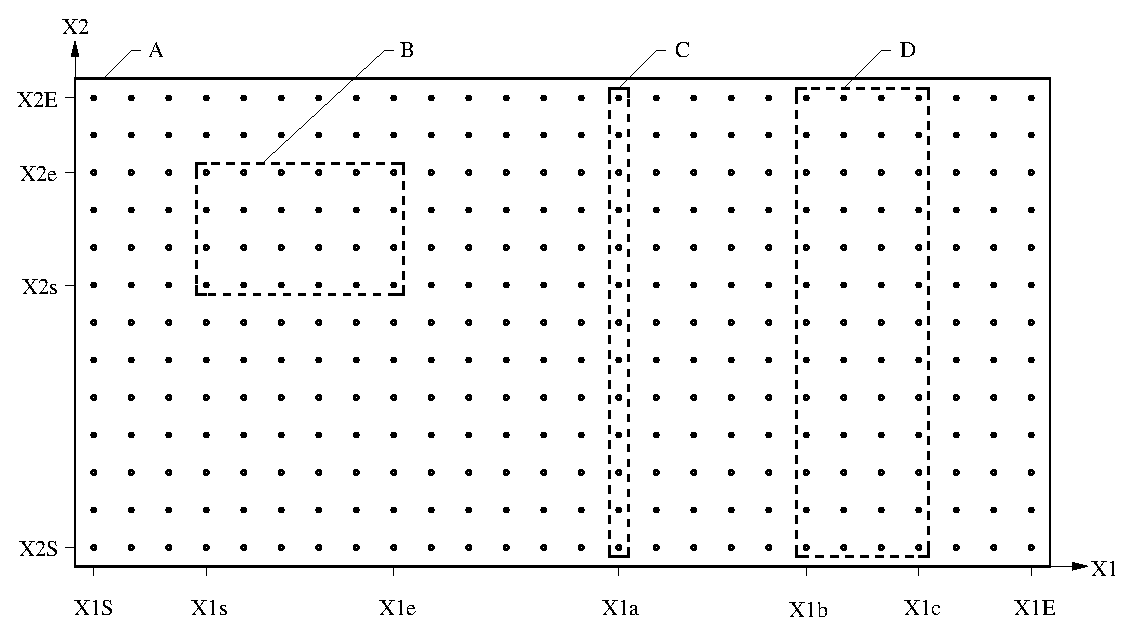
\includegraphics[width=4.7in]{ParentFig3.eps}
   \hspace{1cm}
 \end{center}
\caption{Example of computational domain and subdomain notation in
         two dimensions; the computational
         domain limits are denoted by the superscripts E and S.}
\label{fig:domain-notation}
\end{figure}
%

The acceleration techniques presented in this paper are aimed at reducing
the work needed to solve quasi-hyperbolic or quasi-parabolic systems through the use
of domain decomposition. Nonetheless, the effectiveness of the methods
is not limited to entirely quasi-hyperbolic/parabolic systems and extends to
systems where some regions are quasi-hyperbolic/parabolic
and others strictly elliptic.
It is emphasized that domain decomposition is used here solely as a convergence
acceleration technique, and \emph{does not} modify the discretized residual, the
time stepping schemes, and the convergence criterion, except in the case
of the active-domain method. Convergence is attained
independently of the acceleration technique when
%
\begin{equation}
  \xi \leq \xiverge ~\forall~ {\rm inner~nodes} \, ,
  \label{eqn:convergence_criterion}
\end{equation}
%
with $\xi$ a convergence criterion based on the
maximum between the discretized continuity and energy residuals,
%
\begin{equation}
  \xi\equiv {\rm max} \left(
        \frac{|(R_\Delta)_1|}{ ~\Omega  (U_{\rm ref})_1}~,~...,~
        \frac{|(R_\Delta)_\nf|}{ ~\Omega (U_{\rm ref})_\nf}
  \right) \, ,
\label{eqn:xi}
\end{equation}
%
which is divided by $\Omega U_{\rm ref}$ to obtain units involving only pseudo-time (\ie $\frac{1}{\rm s}$). Note that $U_{\rm ref}$ here does not include the inverse of the metrics Jacobian $\Omega$. Thus $(U_{\rm ref})_1 \sim \rho_{\rm ref}$, $(U_{\rm ref})_{\ns+1}\sim \rho_{\rm ref} a_{\rm ref}$, etc.  
The user-defined convergence threshold $\xiverge$ is typically given a value
of 100 $\frac{1}{\rm s}$, yet this value is not universal
and is dependent on the flowfield at hand.
Based on dimensional analysis arguments, $\xiverge$ can be thought of as the inverse of
a time scale common for all nodes, which we formulate in terms of the free stream
flow speed and a characteristic length, \ie
%
\begin{equation}
 \xiverge \sim \frac{1}{10} \frac{u_\infty}{L_{\rm c}} \, ,
 \label{eqn:xiverge}
\end{equation}
%
where an analogy can be made to the time needed to obtain steady-state
flow using an experimental setup. The characteristic length $L_{\rm c}$
can be taken as the length of the domain for instance.
It is noted, however, that the efficiency of the domain decomposition
methods presented herein is dependent on the precision of $\xi$ as a
convergence criterion, and since this varies from one flow problem to the next,
it might not always be possible to achieve at first the proper compromise between
optimal convergence rate and acceptable accuracy by using Eq.~(\ref{eqn:xiverge}).


Identifying the limits of the computational domain by $X_i^\loopS$ and $X_i^\loopE$
with $i \in [1, ..., \nd]$ and the limits of a subdomain by $X_i^\loops$ and $X_i^\loope$,
with $i \in [1, ..., \nd]$
the region spanned by the subdomain is referred to by the notation
\subdomain{\forall i}{X_i^\loops}{X_i^\loope}, as shown in Fig. \ref{fig:domain-notation}.
For a subdomain with limits different from the computational domain limits in
only one dimension the notation \subdomain{n}{X_n^\loops}{X_n^\loope} is employed,
where it is implied that the limits in the dimensions other than the $n$th do
not differ from those of the computational domain (see Fig. \ref{fig:domain-notation}).
Also, \subdomainshort{n}{X_n^\loops} is a shortcut that stands for the subdomain
\subdomain{n}{X_n^\loops}{X_n^\loops}.
A property that is used in conjunction with the domain decomposition algorithms
is the number of nodes of dependence of the discretized residual, $b_r$, which
is defined as
%
\begin{equation}
 \br \equiv
  \left\{
   \begin{array}{l}
     \begin{array}{l}
       \rm the~maximum~number~of~nodes~on~which~the~discretized\\
       \rm residual~depends~on~each~side~of~the~center~node,
     \end{array}\alb
     \rm or,\alb
     \begin{array}{l}
       \rm half~the~maximum~discretization~stencil~point~minus~one\\
       \rm if~the~stencil~is~symmetric.
     \end{array}
   \end{array}
  \right.
\end{equation}
%
For example, the minmod TVD discretization stencil (which is the longest of all stencils
contained in the residual) would give $\br=2$ but should a first order Roe scheme
be employed instead, then $\br$ would be set to one.
Similarly, the number of nodes of dependence of the boundary nodes is defined as
%
\begin{equation}
\bb \equiv
 \left\{
    \begin{array}{l}
      \rm the~maximum~number~of~nodes~any~boundary~node~depends\\
      \rm on~along~one~direction,
    \end{array}
 \right.
\end{equation}
%
which is set to 2, since
the properties at the boundary nodes are extrapolated from at most 2 inner nodes
using a blend of zeroth and first order extrapolation polynomials.


When the nodes comprised in the subdomain \subdomain{\forall i}{X_i^\loops}{X_i^\loope} are
updated in pseudo-time, then it follows from the definition of $\bb$
that the boundary nodes situated inside \subdomain{\forall i}{X_i^\loops-\bb}{X_i^\loope +\bb}
must be updated. The residual, which depends on both inner and boundary nodes
must then be updated between \subdomain{\forall i}{X_i^\loops-\bb-\br}{X_i^\loope +\bb+\br}.
In many cases where there are no boundary nodes situated in the region
\subdomain{\forall i}{X_i^\loops-\bb}{X_i^\loope+\bb}, it is sufficient to update the residual
in \subdomain{\forall i}{X_i^\loops-\br}{X_i^\loope+\br}. For all methods presented in this
paper, however, this shortcut is not implemented.



\section{Standard Cycle}

The ``standard cycle'' here implies the usual way of updating the solution
in pseudo-time, by first finding the residual for all nodes and then updating
the solution. The algorithm can be written in the following steps:
%
\begin{enumerate}
  \item{update the boundary nodes in the domain\
        \subdomain{\forall i}{X^{\loopS}_i}{X^{\loopE}_i},}
  \item{update the residual in the domain
        \subdomain{\forall i}{X^{\loopS}_i}{X^{\loopE}_i}, }
  \item{update $U$ (by pseudo-time stepping) in \
        the domain \subdomain{\forall i}{X^{\loopS}_i}{X^{\loopE}_i}, and,}
  \item{convergence is attained when $\xi \leq \xiverge$ in the domain \subdomain{\forall i}{X^{\loopS}_1}{X^{\loopE}_1}.}
\end{enumerate}
%



\section{Multizone Cycle}
\label{section:multizone}

One strategy towards improving the standard cycle is to divide the computational
domain into a number of non-overlapping zones of approximately equal size
and to update in pseudo-time only the zones where $\xi>\xiverge$, as first outlined by Parent and Sislian in Ref.\ \cite{jcp:2002:parent}.
A similar stratagem has been previously employed
by Sawley \etal \cite{misc:1994:sawley}
as a convergence acceleration technique for supersonic flows, but where the
computational domain is split into several blocks, instead of several zones. 
Note that a ``zone'' is defined as a computational domain region that
can be bounded by boundary and/or inner nodes (see for example Ref.\
\cite{jcp:1994:rosenfeld}),
while a ``block'' is defined as a region delimitated  by boundary nodes only.
The zone length in each dimension is set to at most $\phi_1$, a user
specified constant usually given a value of 20.
At each iteration, should the maximum $\xi$ inside each zone be greater
than the user-specified threshold $\xiverge$, the inner nodes up to the
zone boundaries are updated in pseudo-time,
followed by the update of the boundary nodes up to the zone boundaries expanded by $\bb$,
and the update of the residual up to the zone boundaries expanded by $\bb+\br$.
The residual and properties of all other nodes of the computational domain
are not altered. Prior to the first iteration,
the computational domain is divided into a number of non-overlapping zones
of length in each dimension no greater than $\phi_1$ with
each zone $z$ defined by the subdomain \subdomain{\forall i}{X^{z,\loops}_i}{X^{z,\loope}_i}.
Then, at each iteration, the following steps are performed:
%
\begin{enumerate}
  \item{for each zone $z$, update $U$ (by pseudo-time stepping) in \
        the subdomain \subdomain{\forall i}{X^{z,\loops}_i}{X^{z,\loope}_i}
	if $\xi > \xiverge$ in the subdomain \subdomain{\forall i}{X^{z,\loops}_i}{X^{z,\loope}_i},}
  \item{for each zone $z$, update the boundary nodes in the subdomain\
        \subdomain{\forall i}{X^{z,\loops}_i-\bb}{X^{z,\loope}_i+\bb}
	if $\xi > \xiverge$ in the subdomain \subdomain{\forall i}{X^{z,\loops}_i}{X^{z,\loope}_i},}
  \item{for each zone $z$, update the residual in the subdomain
        \subdomain{\forall i}{X^{z,\loops}_i-\bb-\br}{X^{z,\loope}_i+\bb+\br}
	if $\xi > \xiverge$ in the subdomain \subdomain{\forall i}{X^{z,\loops}_i}{X^{z,\loope}_i}, and, }
  \item{convergence is attained when $\xi \leq \xiverge$ in the domain \subdomain{\forall i}{X^{\loopS}_1}{X^{\loopE}_1}.}
\end{enumerate}
%
It is noted that the multizone cycle ensures
the residual on all nodes to be up to date after each iteration but,
due to the non self-starting property of this cycle, it is
necessary to compute the residual on the entire domain before the first iteration
is performed.




\section{Active-Domain Cycle}
\label{section:active_domain}


%
\begin{figure}[t]
 \begin{center}
   \fontfig
   \psfrag{X1}[l][l][1][0]{$X_1$}
   \psfrag{X2}[b][b][1][0]{$X_2$}
   \psfrag{X1S}[b][b][1][0]{$X_1^\loopS$}
   \psfrag{X1E}[b][b][1][0]{$X_1^\loopE$}
   \psfrag{X1s}[b][b][1][0]{$X_1^\loops$}
   \psfrag{X1e}[b][b][1][0]{$X_1^\loope$}
   \psfrag{X2S}[r][r][1][0]{$X_2^\loopS$}
   \psfrag{X2E}[r][r][1][0]{$X_2^\loopE$}
   \psfrag{A}[bl][bl][1][0]{\subdomain{\forall i}{X_i^\loopS}{X_i^\loopE}}
   \psfrag{D}[][][1][0]{active-domain}
   \psfrag{E}[][][1][0]{$\begin{array}{c}\rm initial \\ \rm conditions\end{array}$}
   \psfrag{F}[][][1][0]{$\begin{array}{c}\rm residual~monitor\\ \rm subdomain\end{array}$}
   \psfrag{G}[][][1][0]{$M_1<1.001$}
   \psfrag{H}[lt][lt][1][0]{$\begin{array}{l} (\phi_3-\phi_0-1) {\rm ~ nodes} \\ M_1\geq 1.001\end{array}$}
   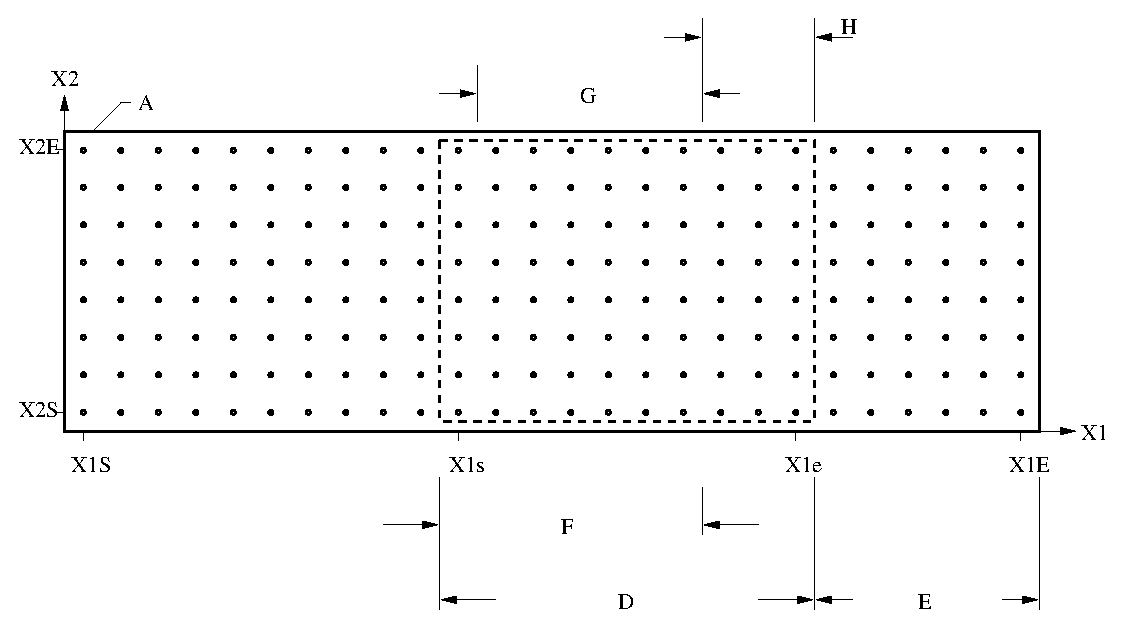
\includegraphics[width=4.7in]{ParentFig4.eps}
 \end{center}
\caption{Schematic of the active-domain cycle with the upstream and downstream boundaries
         in equilibrium including an embedded subsonic region; $\phi_0$ is the minimum
         width of the residual monitor subdomain and $\phi_3$ is the minimum width
         of the active-domain (when no subsonic region is present).}
\label{fig:active-domain}
\end{figure}
%


The ``active-domain'' is an algorithm aimed at decreasing the work needed for
convergence of supersonic inviscid flow \cite{aiaa:1997:nakahashi} and
refers to a band-like computational domain marching in the flow direction
in which localized pseudo-time stepping is performed. The domain width
automatically adjusts to the size of subsonic regions when encountered by
monitoring the streamwise component of the Mach number, as shown in Fig.~\ref{fig:active-domain}.
In our notation, the active-domain algorithm can be written as follows,
denoting the left boundary of the computational window by $X_1^{\loops}$
and the right boundary by $X_1^{\loope}$:
%
\begin{enumerate}
  \item{update the boundary nodes in the subdomain \subdomain{1}{X^{\loops}_1}{X^{\loope}_1},}
  \item{update the residual in the subdomain \subdomain{1}{X^{\loops}_1}{X^{\loope}_1},}
  \item{update $U$ (by pseudo-time stepping) in the subdomain \subdomain{1}{X^{\loops}_1}{X^{\loope}_1},}
  \item{redefine the active-domain boundaries:}
  \begin{enumerate}
  \item{if $M_1<1.001$ for any node in the
        subdomain \subdomain{1}{X^{\loops}_1}{X^{\loops}_1}
        then decrease $X_1^{\loops}$ by one,}
  \item{if $M_1<1.001$ for any node in the
        subdomain \subdomain{1}{X^{\loope}_1-(\phi_3-\phi_0)}{X^{\loope}_1}
        then increment $X_1^{\loope}$ by one,}
  \item{if $\xi \leq \xiverge$ for all nodes in the subdomain
       \subdomain{1}{X^{\loops}_1}{X^{\loope}_1-(\phi_3-\phi_0)}
       then increment $X^{\loope}_1$ by $\phi_0$ and set $X^{\loops}_1=X^{\loope}_1-\phi_3$,
       and,}
  \end{enumerate}
  \item{convergence is attained when $\xi \leq \xiverge$ for all nodes in the subdomain \subdomain{1}{X^{\loops}_1}{X^{\loope}_1}
        and when $X^{\loope}_1=X^{\loopE}_1$.}
\end{enumerate}
%
The size of the residual-monitor region $\phi_0$ and the size of the active-domain
$\phi_3$ are user-specified constants typically given values of 4 and 9 respectively.
It is emphasized that the active-domain is restricted to inviscid flow
due to the ``ellipticity sensors'' in Steps 4a and 4b being based on the streamwise
component of the Mach number. For viscous flows, this would effectively
enlarge the active-domain to the size of any object due to the vanishing
value of the Mach number in the vicinity of a wall.
Aside from being restricted to inviscid flow,
the active-domain algorithm does not guarantee
that $\xi \leq \xiverge$ for all nodes of the computational domain when convergence
is attained. This is due to the assumption in Step~4a that
streamwise ellipticity is present locally only when the streamwise component of
the Mach number is less than 1. For inviscid flow, this is exactly true if
the discretization stencil of the streamwise
convection derivative is upwinded (such as the first-order accurate Roe scheme for
instance),  but is not true for the Yee-Roe scheme used herein due to the Yee
flux limiter being a function of downstream nodes, even when the flow is locally
supersonic.
Therefore, when used in conjunction with a flux-limiter inducing streamwise
ellipticity in supersonic flow, the active-domain
does not meet the necessary convergence criterion for a
well-posed acceleration technique [as stated previously in
Eq.~(\ref{eqn:convergence_criterion})].




\section{Marching-Window Cycle}
\label{section:marching-window}
%
\begin{figure}[t]
 \begin{center}
   \fontfig
   \psfrag{X1}[l][l][1][0]{$X_1$}
   \psfrag{X2}[b][b][1][0]{$X_2$}
   \psfrag{X1S}[b][b][1][0]{$X_1^\loopS$}
   \psfrag{X1E}[b][b][1][0]{$X_1^\loopE$}
   \psfrag{X1s}[b][b][1][0]{$X_1^\loops$}
   \psfrag{X1e}[b][b][1][0]{$X_1^\loope$}
   \psfrag{X2S}[r][r][1][0]{$X_2^\loopS$}
   \psfrag{X2E}[r][r][1][0]{$X_2^\loopE$}
   \psfrag{A}[bl][bl][1][0]{\subdomain{\forall i}{X_i^\loopS}{X_i^\loopE}}
   \psfrag{B}[bl][bl][1][0]{\subdomain{1}{X_1^{\rm s}}{X_1^{\rm e}}}
   \psfrag{C}[][][1][0]{$\xi \leq \xiverge$}
   \psfrag{D}[][][1][0]{marching window}
   \psfrag{E}[][][1][0]{$\begin{array}{c}\rm initial\\ \rm conditions\end{array}$}
   \psfrag{F}[r][r][1][0]{$\varphi > \varphiverge$}
   \psfrag{G}[r][r][1][0]{outflow boundary}
   \psfrag{H}[][][1][0]{$\begin{array}{c}\rm \phi_3 nodes\\  \varphi \leq \varphiverge\end{array}$}
   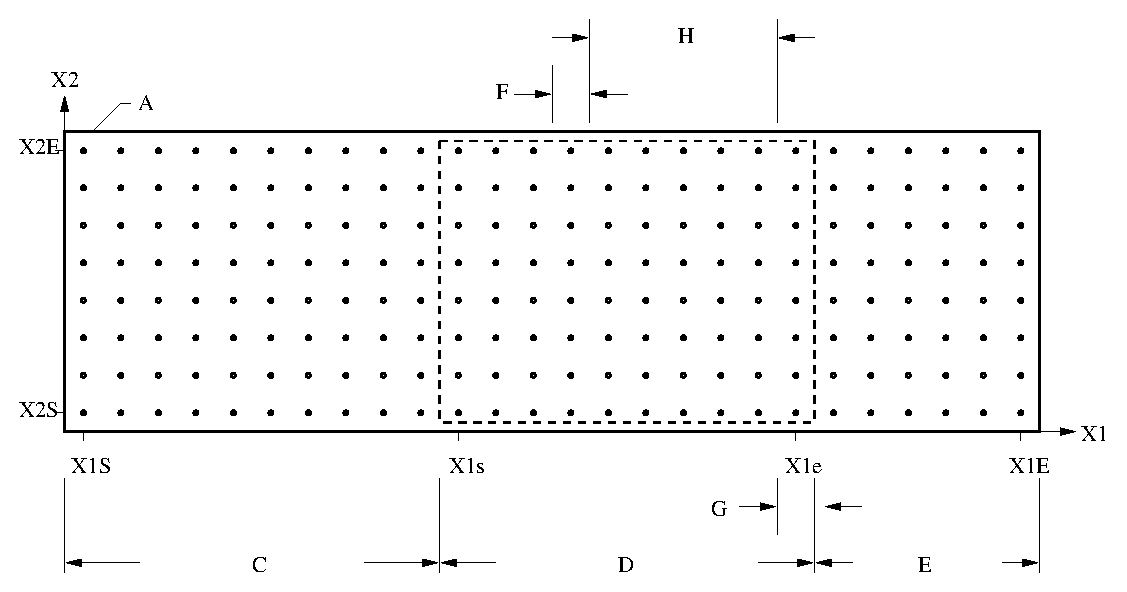
\includegraphics[width=4.7in]{ParentFig5.eps}
 \end{center}
\caption{Schematic of the marching-window cycle with the upstream and downstream boundaries
         in equilibrium including an embedded streamwise elliptic region which
         is bounded upstream by the condition $\xi \leq \xiverge$ and downstream
         by the condition $\varphi\leq \varphiverge$;
         a dynamic outflow boundary condition is forced on
         all inner nodes in \subdomainshort{1}{X_1^\loope}.}
\label{fig:marching-window}
\end{figure}
%

An improvement to the active-domain cycle
that permits the solution of viscous streamwise separated flows and satisfies the
convergence criterion of Eq.~(\ref{eqn:convergence_criterion}) was outlined by Parent and Sislian in Ref.\ \cite{jcp:2002:parent}.
Named the ``marching-window'', the algorithm differs from the active-domain
on three points, namely 1) a dynamic outflow boundary is forced at the downstream
boundary of the marching-window (see Fig.~\ref{fig:marching-window}),
2) the ellipticity sensor responsible for a shift downstream of the downstream
boundary of the marching-window is based on a Vigneron splitting of the streamwise
pressure derivative instead of the streamwise component of the Mach number,
and 3) the upstream boundary of the marching-window is positioned
such that $\xi \leq \xiverge$ for all nodes upstream, instead of being
a function of a residual monitor region and a streamwise ellipticity sensor based on the streamwise component of
the Mach number.
Before the first iteration, the upstream boundary of the marching-window is set to the upstream
boundary of the computational
domain with the downstream boundary of the marching-window
separated from the upstream boundary by $\bb$ nodes.
Denoting the upstream boundary of the marching-window by $X_1^{\loops}$
and the downstream-boundary by $X_1^{\loope}$, the marching-window cycle can
be written as:
%
\begin{enumerate}
  \item{update $U$ (by pseudo-time stepping) in the subdomain \subdomain{1}{X^{\loops}_1}{X^{\loope}_1},}
  \item{update the boundary nodes in the subdomain \subdomain{1}{X^{\loops}_1-\bb}{X^{\loope}_1},}
  \item{update the residual in the subdomain \subdomain{1}{X^{\loops}_1-\bb-\br}{X^{\loope}_1},}
  \item{redefine the marching-window boundaries:}
  \begin{enumerate}
  \item{find the maximum value for $X_1^{\loops}$
        such that $\xi \leq \xiverge$ for all nodes in the
	subdomain \subdomain{1}{X_1^\loopS}{X_1^{\loops}-1},}
  \item{every $\phi_2$ iterations, if $\varphi>\varphiverge$ for any node in the
        subdomain \subdomain{1}{X^{\loope}_1-\phi_3}{X^{\loope}_1} or
	if $X_1^{\loops}>X_1^{\loope}-\phi_3$
        then 1) increment $X_1^{\loope}$ by one,
        2) update the boundary nodes in the subdomain \subdomain{1}{X^{\loope}_1-1-\bb}{X^{\loope}_1}
        and 3) update the residual in the subdomain \subdomain{1}{X^{\loope}_1-1-\bb-\br}{X^{\loope}_1-1},
	and,}
  \end{enumerate}
  \item{convergence is attained when $\xi \leq \xiverge$ for all nodes in the subdomain \subdomain{1}{X^{\loops}_1}{X^{\loope}_1}
        and when $X^{\loope}_1=X^{\loopE}_1$.}
\end{enumerate}
%
The marching-window cycle is not self-starting and it must be ensured that the residual is
updated for all nodes part of the computational window before the first iteration.

The ability of the marching-window at satisfying the convergence criterion of
Eq.~(\ref{eqn:convergence_criterion}) lies in Steps 1-3, where $U$ is updated in
pseudo-time in Step~1 \emph{before} determining the residual in Step~3. Once $U$
is updated in Step~1 on the subdomain \subdomain{1}{X^{\loops}_1}{X^{\loope}_1}, since
a boundary node depends on at most $\bb$ neighbors, it is sufficient to update
the boundary nodes in the subdomain \subdomain{1}{X^{\loops}_1-\bb}{X^{\loope}_1}
to guarantee that all boundary nodes upstream of $X^{\loope}_1$ are up to date
after Step~2.
Once the boundary nodes have been updated in the subdomain
\subdomain{1}{X^{\loops}_1-\bb}{X^{\loope}_1}, since the discretized residual depends
on at most $\br$ neighbours, it is sufficient to update the residual in the
subdomain \subdomain{1}{X^{\loops}_1-\bb-\br}{X^{\loope}_1} to guarantee that the
residual of all nodes upstream of $X^{\loope}_1$ are up to date after Step~3.
Since $\xi$ is a function of the residual, $\xi$ upstream of $X^{\loope}_1$
is up to date, and the upstream boundary of the marching-window $X^{\loops}_1$
can be positioned correctly in Step 4a by ensuring for all nodes upstream
of $X^{\loope}_1$ that $\xi\leq\xiverge$. This serves two purposes: 1) the convergence
criterion of Eq.~(\ref{eqn:convergence_criterion}) is satisfied if convergence
is attained in Step~5, and 2) the upstream boundary of the marching-window
moves upstream for any upstream propagating wave that affects the residual significantly
and raises $\xi$ above the user-defined accuracy threshold $\xiverge$. Contrarily
to the active-domain, the upstream propagating wave is not limited to locally
subsonic flow but includes all \emph{significant} streamwise elliptic phenomena,
such as streamwise separated flow, streamwise viscous derivatives, or flux limiters
in the streamwise convection derivative, for instance.

Step 4b advances the marching-window upstream boundary when the width
of the window is smaller than a user-specified constant $\phi_3$, or when
the streamwise ellipticity sensor $\varphi$ is greater than the user-specified
constant $\varphiverge$ for any node part of the subdomain
\subdomain{1}{X^{\loope}_1-\phi_3}{X^{\loope}_1}.
The streamwise ellipticity sensor $\varphi$ is here chosen as the component
of the streamwise convection derivative inducing a streamwise ellipticity.
This is derived, following an approach by Vigneron \etal \cite{aiaaconf:1978:vigneron},
by multiplying by $\zeta$ the effective pressure terms in the momentum fluxes
part of the streamwise convection flux $F_1$. The eigenvalues of the streamwise
convective flux Jacobian with $\zeta$ frozen can then be shown to correspond to:
%
\begin{displaymath}
 \wtilde{\lambda}_1=
 \left[
   V_1,~
   V_1,~
   \rightarrow,~
   V_1 + \frac{1}{2} V_1 P_{\rho E} \left(1-\zeta\right)
       + \wtilde{a}_1 \widehat{X}_1,~
   V_1 + \frac{1}{2} V_1 P_{\rho E} \left(1-\zeta\right)
       - \wtilde{a}_1 \widehat{X}_1,~
   V_1,~
   V_1
 \right]^{\rm D} 
\end{displaymath}
%
%
\begin{displaymath}
  {\rm with ~~~~~}
  \wtilde{a}_1=\left\{
    \frac{1}{4}\left[
       V_1 P_{\rho E} \left(1-\zeta\right)
    \right] ^2
    +\widehat{X}_1^2 \zeta \left[
       P_\rho+\frac{2}{3} k + P_{\rho E} \left(H-k-q^2\right)
    \right]
  \right\}^{\frac{1}{2}} \, .
\end{displaymath}
%
Then, for all the eigenvalues to share the same sign (a necessary condition
for an hyperbolic system), it is required that
%
\begin{equation}
  \zeta=\min\left(
    1,~~
    V_1^2 \frac{1+P_{\rho E}}{\widehat{X}_1^2 a^2+V_1^2 P_{\rho E}}
  \right)
  =\min\left(
    1,~~
    \frac{M_1^2(1+P_{\rho E})}{1+M_1^2 P_{\rho E}}
  \right)
\end{equation}
%
where the streamwise Mach number $M_1$ corresponds to $V_1/a\widehat{X}_1$.
If multiplying by $\zeta$ the pressure derivative terms part of the momentum
components of $\partial F_1 / \partial X_1$ results in a hyperbolic system,
it follows that the component of the streamwise convection derivative
which induces a streamwise ellipticity is $(1-\zeta)$ times the pressure derivative
terms part of the momentum components of $\partial F_1 / \partial X_1$.
The product is then normalized with $\rho a$ to obtain units of inverse pseudo-time:
%
\begin{equation}
  \varphi \equiv
      \bigfrac{1}{\rho a}
        \left\{ \sum_{j=1}^\nd
          \left[
            (1-\zeta) X_{1,j} \bigfrac{\partial P^\star}{\partial X_1}
          \right]^2
        \right\}^{\frac{1}{2}}
          =
      \bigfrac{\widehat{X}_1}{\rho a} \max \left( 0, ~ \bigfrac{1-M_1^2}{1+P_{\rho E} M_1^2} \right)
        \left| \bigfrac{\partial P^\star}{\partial X_1}\right| \, .
  \label{eqn:varphi}
\end{equation}
%
The ellipticity sensor $\varphi$ makes two important assumptions:
1) the streamwise ellipticity originating from the streamwise viscous derivative
   terms and the flux limiter part of the streamwise convection derivative is
   assumed negligible, and
2) at the point where $\varphi$ is evaluated, the solution is assumed to be converged
   to steady-state.
The first assumption is remedied by introducing a minimum width of the marching-window,
$\phi_3$, which is typically given a value ranging from 9 to 15.
The second assumption
can lead to some performance degradation of the marching-window
when the flow near the downstream boundary is far from convergence. For this reason,
the user-adjustable parameter $\phi_2$ is introduced in Step~4a, with the consequence
of evaluating $\varphi$ every $\phi_2$ iterations only.
Therefore, a high value given to $\phi_2$ helps in ensuring a
more converged solution near the downstream boundary, and reduces the error
in the ellipticity sensor $\varphi$ due to temporarily non steady-state flow.
It is suggested to give the ellipticity sensor threshold, $\varphiverge$,
a value of about 100 times the one given to $\xiverge$, that is,
%
\begin{equation}
  \varphiverge \sim 10~\frac{u_\infty}{L_{\rm c}} \, ,
  \label{eqn:varphiverge}
\end{equation}
%
with $L_{\rm c}$ a characteristic length of the system. In Step~4b, after
the downstream boundary of the marching-window is advanced by one station,
the update of the boundary
nodes in the subdomain \subdomain{1}{X^{\loope}_1-1-\bb}{X^{\loope}_1} and
of the residual in the subdomain \subdomain{1}{X^{\loope}_1-1-\bb-\br}{X^{\loope}_1-1}
is necessary to ensure that the residual is properly updated in the marching-window,
which is necessary for Step~1 to be performed correctly at the following iteration.

While the user-definable constants $\phi_2$, $\phi_3$, and $\varphiverge$ affect
the performance of the marching-window cycle as a convergence acceleration technique,
they do \emph{not} affect the accuracy of the solution when convergence is attained
due to the convergence criterion of Eq.~(\ref{eqn:convergence_criterion}) being
satisfied.


\section{Multizone-Marching Cycle}

The performance of the marching-window algorithm can be enhanced by introducing
multizone decomposition inside the marching-window \cite{jcp:2002:parent}. Before each iteration,
the marching-window subdomain \subdomain{1}{X^{\loops}_1}{X^{\loope}_1}
is decomposed into several zones of length no more than $\phi_1$ nodes in each dimension. Then,
Steps~1-3 of the marching-window cycle (see Section~\ref{section:marching-window})
are replaced by Steps~1-3 of the multizone cycle (see Section~\ref{section:multizone}).


\section{Multizone-Sweeping Cycle}

Intended for time-accurate simulations using dual-time stepping,
the sweeping-window algorithm \cite{jcp:2002:parent} is identical to the marching-window
algorithm, with the exception of no outflow boundary condition forced on the downstream
boundary of the sweeping-window. When the converged solution of the previous
time level is used as initial conditions for the current time level, not forcing
an outflow condition at the downstream boundary helps in attaining faster
convergence due to the initial conditions providing a better ``guess'' at the downstream boundary.
For the same reasons, the sweeping-window cycle can also be used to gain extra
orders of magnitude of convergence on the solution obtained by the marching-window.


  \bibliographystyle{warpdoc}
  \bibliography{all}


\end{document}














